\documentclass{beamer}
%Information to be included in the title page:


\usepackage{listings}
\usepackage{color}
\usepackage{xcolor}
\usepackage{graphicx}
\usepackage{tikz}
\definecolor{mygreen}{rgb}{0,0.6,0}
\definecolor{mygray}{rgb}{0.5,0.5,0.5}
\definecolor{mymauve}{rgb}{0.58,0,0.82}
\definecolor{codegreen}{rgb}{0,0.6,0}
\definecolor{codegray}{rgb}{0.5,0.5,0.5}
\definecolor{codepurple}{rgb}{0.58,0,0.82} 
\definecolor{backcolour}{rgb}{0.95,0.95,0.92}
\lstset{language=Python,keywordstyle={\bfseries \color{blue}}}
\lstset{ %
  backgroundcolor=\color{white},   % choose the background color
  basicstyle=\footnotesize,        % size of fonts used for the code
  breaklines=true,                 % automatic line breaking only at whitespace
  captionpos=b,                    % sets the caption-position to bottom
  commentstyle=\color{mygreen},    % comment style
  escapeinside={\%*}{*)},          % if you want to add LaTeX within your code
  keywordstyle=\color{blue},       % keyword style
  stringstyle=\color{mymauve},     % string literal style
  backgroundcolor=\color{backcolour},   
    commentstyle=\color{codegreen},
    keywordstyle=\color{magenta},
    numberstyle=\tiny\color{codegray},
    stringstyle=\color{codepurple},
    basicstyle=\ttfamily\footnotesize,
    breakatwhitespace=false,         
    breaklines=true,                 
    captionpos=b,                    
    keepspaces=true,                 
    numbers=left,                     
    numbersep=5pt,                  
    showspaces=false,                
    showstringspaces=false,
    showtabs=false,                  
    tabsize=2
}
\title{Solving Mazes Computationally in Python}
\author{Sanjay Seshan and Bill Wang}
\institute{MIT Splash}
\date{20 November 2022}

% \usepackage{listings}
\usetikzlibrary{arrows.meta, automata, positioning, quotes}

\begin{document}

\frame{\titlepage}

\begin{frame}
\frametitle{The Problem}
\begin{itemize}
    \item We consider a maze to be a series of paths from a start position to an end position
    \item Mazes are both traditional puzzles in newspapers and much larger
    \item The concept of solving a maze is simple, but often hard by hand
    \item How can we scale this on a computer?
    
    
\includegraphics[width=5cm]{figures/lgg_graph.jpg}
\end{itemize}

\end{frame}

\begin{frame}
    \frametitle{Basic Algorithm}
    Let's consider the following maze.
    \begin{itemize}
        \item Solve this using a right hand rule method/follow the wall
        \item This is a trivial approach -- follow a single wall until the end.
        
    \end{itemize}

    
\includegraphics[width=5cm]{figures/maze_bfs_lg.png}

    
    \end{frame}


\begin{frame}
    \frametitle{Basic Algorithm}
    Let's consider the following maze.
    \begin{itemize}
        \item Solve this using a right hand rule method/follow the wall
        \item This is a trivial approach -- follow a single wall until the end.
        
    \end{itemize}

    
\includegraphics[width=5cm]{figures/maze_bfs_lg_rhr.png}

    
    \end{frame}

    \begin{frame}
        \frametitle{DFS Algorithm}
        Let's consider the following maze.
        \begin{itemize}
            \item Solve this by considering all outgoing paths at each intersection
            \item Select one and continue, unless a dead-end is found
            \item Backtrack and try again until the exit is reached
            \item This is called Depth First Search (DFS)
            
        \end{itemize}
    
        
\includegraphics[width=5cm]{figures/maze_bfs_lg.png}
    
        
        \end{frame}


        \begin{frame}
            \frametitle{DFS Algorithm}
            Let's consider the following maze.
            \begin{itemize}
                \item What patterns do you notice? Does this give you the ``best'' path? 
                \item Is there a better path?
                \item Which is the ``shortest'' path?


            \end{itemize}
        
            
\includegraphics[width=5cm,scale=2]{../dfs_out.png}
        
            
            \end{frame}
            \begin{frame}[fragile]
                \frametitle{DFS Algorithm}
\begin{lstlisting}
procedure DFS(G, v) is
    label v as discovered
    for all directed edges from v to w that are in G.adjacentEdges(v) do
        if vertex w is not labeled as discovered then
            recursively call DFS(G, w)
\end{lstlisting}

            \end{frame}

            \begin{frame}[fragile]
                \frametitle{DFS Algorithm}
\begin{lstlisting}
def run_dfs(pixels,curr,visited):
    for dr, dc in [(1,0),(-1,0),(0,1),(0,-1)]:
        visited.add(curr)
        new = curr[0] + dr, curr[1] + dc
        if new[0] < rdim and new[1] < cdim and new[0] >=0 and new[1] >=0:
            if pixels[new[0],new[1]] == red:
                return (curr,new)
            elif pixels[new[0],new[1]] == white:
                if new not in visited:
                    res = run_dfs(pixels, new, visited)
                    if res is not None:
                        return (curr,)+res
                    else:
                        visited.remove(curr)
    return None
pos = run_dfs(pixels,(0,1),set())\end{lstlisting}

            \end{frame}

            \begin{frame}
                \frametitle{BFS Algorithm}
                Let's consider the following maze.
                \begin{itemize}
                    \item Solve this by considering all outgoing paths at each intersection
                    \item Try each path
                    \item Cancel paths that do not work
                    \item This is called Breath First Search (BFS)
                    \item This is hard to do by hand so we will do it computationally
    
                \end{itemize}
                
\includegraphics[width=5cm]{figures/maze_bfs_lg.png}

                % 
\includegraphics[width=5cm,scale=2]{../bfs_out.png}
            
                
                \end{frame}
    

                

            \begin{frame}
                \frametitle{BFS Algorithm}
                Let's consider the following maze.
                \begin{itemize}
                    \item This looks much better
    
                \end{itemize}
                % 
\includegraphics[width=5cm]{figures/maze_bfs_lg.png}

                
\includegraphics[width=5cm,scale=2]{../bfs_out.png}
            
                
                \end{frame}
                \begin{frame}[fragile]
                    \frametitle{BFS Algorithm}
    \begin{lstlisting}
procedure BFS(G, root) is
    let Q be a queue
    label root as explored
    Q.enqueue(root)
    while Q is not empty do
        v := Q.dequeue()
        if v is the goal then
            return v
        for all edges from v to w in G.adjacentEdges(v) do
            if w is not labeled as explored then
                label w as explored
                w.parent := v
                Q.enqueue(w)
\end{lstlisting}
    
                \end{frame}


                \begin{frame}[fragile]
                    \frametitle{BFS Algorithm}
    \begin{lstlisting}
def run_bfs(pixels,rdim, cdim):
    Q = [((0,1),)]
    while Q != []:
    path = Q.pop(0)
    curr = path[-1]
    for dr, dc in [(1,0),(0,1),(-1,0),(0,-1)]:
        new = curr[0] + dr, curr[1] + dc
        if  new[0] < rdim and new[1] < cdim and new[0] >=0 and new[1] >=0:
        if pixels[new[0],new[1]] == red:
            return path+(new,)
        elif pixels[new[0],new[1]] == white:
            if new not in path:
                new_path = path+(new,)
                Q.append(new_path)
\end{lstlisting}
    
                \end{frame}


                \begin{frame}[fragile]
                    \frametitle{Expanded Problem -- Train routes in Europe}
\begin{itemize}
    \item What is the shortest path from London to Metz? Consider this as a maze with different distances between cities.

    \item In terms of stops? 

    \item In terms of distance? 

    \item Assume all trains are the same speed and there is no time lost between stops. 

    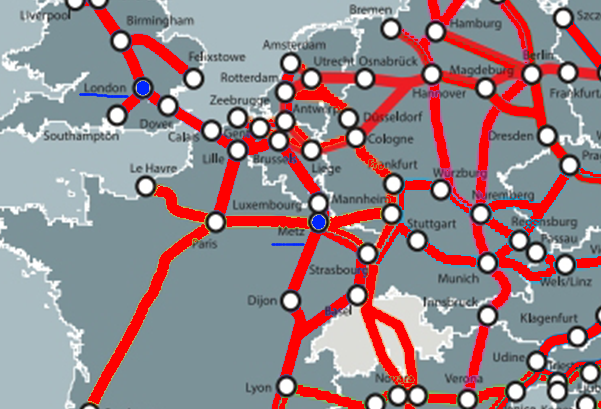
\includegraphics[width=7cm]{figures/london_trains.png}

\item Are all stops evenly spaced? What is ``shortest'' here?
\end{itemize}

\end{frame}


\begin{frame}[fragile]
    \frametitle{Expanded Problem -- Train routes in Europe}
\begin{itemize}
\item What is the shortest path from London to Metz?

\item In terms of stops? (BFS)

\textit{London to Dover to Calais to Lille to Paris to Metz}

\item In terms of distance? 

\textit{London to Dover to Calais to Lille to Brussels to Luxembourg to Metz}

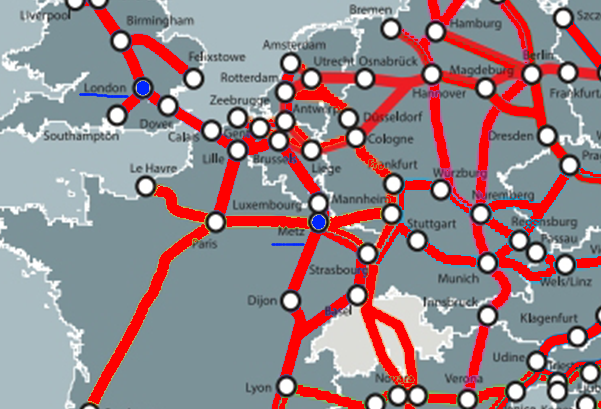
\includegraphics[width=7cm]{figures/london_trains.png}

\end{itemize}

\end{frame}



\begin{frame}[fragile]
    \frametitle{Mazes to Graphs}

\begin{itemize}
    \item 
Finding a path for trains is similar to solving a maze -- there are possible routes and forks that must be followed 
\item How can we convert a maze to a graph? What is an intersection? What is a path?
\item Each node is a "vertex" and each path is an "edge", edges can be directed. Solving paths in graphs is similar to solving mazes. The same algorithms apply.
\end{itemize}


Intersection:

    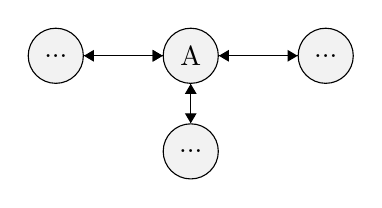
\begin{tikzpicture}[
node distance = 5mm and 10mm,
every state/.append style = {inner sep=0pt, fill=gray!10,
                             minimum size=7mm},
every edge/.style = {draw, -Triangle, bend angle=15},
                auto=right,
                        ]
\node (s1) [state]         {...};
\node (s2) [state, right=of s1]   {A};
\node (s3) [state, below=of s2]         {...};
% \node (s4) [state,  right=of s3]   {C};
\node (s5) [state, right =of s2]   {...};
\draw   (s1) edge [""]             (s2)
(s1) edge [""]             (s2)
(s2) edge [""]             (s1)
(s2) edge [""]             (s3)
(s3) edge [""]             (s2)
% (s4) edge [""]             (s5)
(s5) edge [""]             (s2)
(s2) edge [""]             (s5);
% (s4) edge [""]             (s3)
   \end{tikzpicture}
                
   Standard path:

   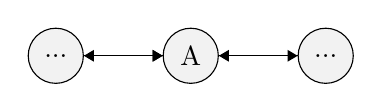
\begin{tikzpicture}[
    node distance = 5mm and 10mm,
    every state/.append style = {inner sep=0pt, fill=gray!10,
                                 minimum size=7mm},
    every edge/.style = {draw, -Triangle, bend angle=15},
                    auto=right,
                            ]
    \node (s1) [state]         {...};
    \node (s2) [state, right=of s1]   {A};
    % \node (s3) [state, below=of s2]         {D};
    % \node (s4) [state,  right=of s3]   {C};
    \node (s5) [state, right =of s2]   {...};
    \draw   (s1) edge [""]             (s2)
    (s1) edge [""]             (s2)
    (s2) edge [""]             (s1)
    % (s2) edge [""]             (s3)
    % (s3) edge [""]             (s2)
    % (s4) edge [""]             (s5)
    (s5) edge [""]             (s2)
    (s2) edge [""]             (s5);
    % (s4) edge [""]             (s3)
       \end{tikzpicture}
%    This is called Dijkstra's algorithm.

%    Can we represent the above map, or a maze, like this?


\end{frame}


\begin{frame}[fragile]
    \frametitle{Dijkstra's Algorithm}

\begin{itemize}
    \item 
    Consider a reduced representation -- what is the shortest path from E to D?

\item Let the number on the arrow be the distance from each node or city. 
\item The direction of the arrow maps the direction of travel permitted. 
\item What pattern do you see? 
\end{itemize}

    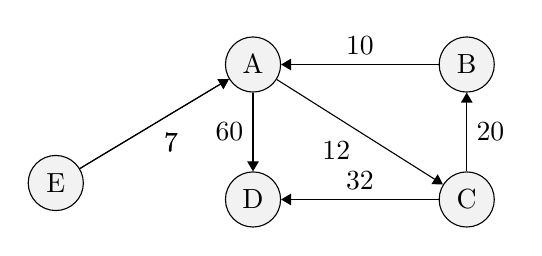
\begin{tikzpicture}[
node distance = 10mm and 20mm,
every state/.append style = {inner sep=0pt, fill=gray!10,
                             minimum size=7mm},
every edge/.style = {draw, -Triangle, bend angle=15},
                auto=right,
                        ]
\node (s1) [state]         {E};
\node (s2) [state, above right=of s1]   {A};
\node (s3) [state, below=of s2]         {D};
\node (s4) [state,  right=of s3]   {C};
\node (s5) [state, above =of s4]   {B};
\draw   (s1) edge ["7"]             (s2)
(s1) edge ["7"]             (s2)
(s2) edge ["12"]             (s4)
(s2) edge ["60"]             (s3)
(s4) edge ["20"]             (s5)
(s5) edge ["10"]             (s2)
(s4) edge ["32"]             (s3);
   \end{tikzpicture}
                
%    This is called Dijkstra's algorithm.

%    Can we represent the above map, or a maze, like this?


\end{frame}

\begin{frame}[fragile]
    \frametitle{Dijkstra's Algorithm}

\begin{itemize}
    \item 
    Consider a reduced representation -- what is the shortest path from E to D?

    \textit{E to A to C to D}

    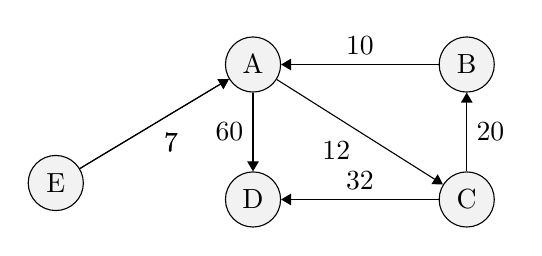
\begin{tikzpicture}[
node distance = 10mm and 20mm,
every state/.append style = {inner sep=0pt, fill=gray!10,
                             minimum size=7mm},
every edge/.style = {draw, -Triangle, bend angle=15},
                auto=right,
                        ]
\node (s1) [state]         {E};
\node (s2) [state, above right=of s1]   {A};
\node (s3) [state, below=of s2]         {D};
\node (s4) [state,  right=of s3]   {C};
\node (s5) [state, above =of s4]   {B};
\draw   (s1) edge ["7"]             (s2)
(s1) edge ["7"]             (s2)
(s2) edge ["12"]             (s4)
(s2) edge ["60"]             (s3)
(s4) edge ["20"]             (s5)
(s5) edge ["10"]             (s2)
(s4) edge ["32"]             (s3);
   \end{tikzpicture}
      
   \item Instead of considering each branch equally like in BFS, we consider the edge weight by taking the lowest one so far at each branch
\item  This is called Dijkstra's algorithm.

\item    Can we represent the above map, or a maze, like this?
\end{itemize}


\end{frame}


\begin{frame}[fragile]
    \frametitle{Dijkstra's Algorithm}

%     for each vertex v in Graph.Vertices:
%     dist[v] ← INFINITY
%     prev[v] ← UNDEFINED
%     add v to Q
% dist[source] ← 0

% if alt < dist[v]:
%                     dist[v] ← alt
%                     prev[v] ← u

\begin{lstlisting}
function Dijkstra(Graph, source):
    while Q is not empty:
            u <- vertex in Q with min dist[u]
            remove u from Q
            
            for each neighbor v of u still in Q:
                alt <- dist[u] + Graph.Edges(u, v)
                push (prev[v] <- u with dist[v] <- alt) to Q

        if u is target:
            return path prev[]
   
\end{lstlisting}

\end{frame}



\begin{frame}[fragile]
    \frametitle{Dijkstra's Algorithm}
\begin{lstlisting}
def run_dijkstra(nodes):
    Q = [((nodes[0],),0)]
    while Q != []:
        imin = 0
        vmin = None
        for i in range(len(Q)):
            if vmin is None or Q[i][1] < vmin:
                vmin = Q[i][1]
                imin = i
        path, dist = Q.pop(imin)
        curr = path[-1]
        for child, next_dist in curr.get_children():
            if child == nodes[-1]:
                return path+(child,)
            elif child not in path:
                new_path = path+(child,)
                Q.append((new_path,dist+next_dist))
\end{lstlisting}

\end{frame}


\begin{frame}
    \frametitle{Demos}

    \begin{enumerate}[(1)]
        \item Simple maze using DFS
        \item Simple maze using BFS
        \item Large maze using BFS
        \item Simple graph using Dijkstra's algorithm
        \item Map of European trains using Dijkstra's algorithm
        \item Map of Cambridge using Dijkstra's algorithm
    \end{enumerate}

\end{frame}

\begin{frame}
    \frametitle{Discussion}

    \begin{enumerate}[(1)]
        \item How can we use a graph to represent a maze?
        \item How can we scale graphs to solve large problems?
        \item How does solving mazes apply to the real world?
        \item How fast do these run? Can we make them faster?
    \end{enumerate}

\end{frame}


\begin{frame}
    \frametitle{Discussion}

    \begin{enumerate}[(1)]
        \item How can we use a graph to represent a maze?
        
        \textit{Consider each position as a vertex and connecting positions as vertices}
        \item How can we scale graphs to solve large problems?
        
        \textit{Represent large data as a graph that can be solved -- perhaps reduce to small problems and expand}

        \item How does solving mazes apply to the real world?

        \textit{Finding routes uses graph algorithms in effect. Think Google Maps.}

        \item How fast do these run? Can we make them faster?

        \textit{For those curious, our examples are inefficient, but we can make these run in $O(|V|+|E|)$ time for BFS and DFS and $O(|E| + |V|\log |V|)$ time for Dijkstra's (E is the number of edges and V vertices). We can improve our array operations by using more advanced algorithms and data structures. We can create a better representation of grids. This is more for another class.}

    \end{enumerate}

\end{frame}

\begin{frame}[fragile]
    \frametitle{Reference}

\begin{lstlisting}
class Node(object):
    def __init__(self, name):
        self.children = []
        self.name = name
    def add_connection(self, child, distance):
        self.children.append((child,distance))
    def get_children(self):
        return self.children
    def __repr__(self):
        return self.name
E = Node("E")
A = Node("A")
D = Node("D")
C = Node("C")
B = Node("B")
mini = [E,A,C,B,D]
E.add_connection(A,7)
D.add_connection(A,60)
A.add_connection(C,12)
C.add_connection(B,20)
B.add_connection(A,10)
C.add_connection(D,32)
    \end{lstlisting}
\end{frame}
    \begin{frame}[fragile]
        \frametitle{Reference}
    
    \begin{lstlisting}
from PIL import Image

im = Image.open("maze_bfs.png")

pixels = im.load()

rdim, cdim = im.size

red = (255,0,0, 255)
blue = (0,0,255, 255)
white = (255,255,255, 255)
black = (0,0,0, 255)
    \end{lstlisting}
    
    \url{https://github.com/sanjayseshan/mit-splash-mazes}
\end{frame}

\end{document}